\scanpage{13}
\mspage{12}
\mspage{IV-\unsure{963}}

\uline{briques séparables de} $\kappa(\underline p)$ (ce qui entraîne que les fibres du morphisme canonique $\operatorname{Spec}({}^{\mathrm{hs}}A)\to\operatorname{Spec}(A)$ sont \uline{géométriquement régulières}).

\uline{Corollaire} (18.8.\deleted{9}\inserted{12}).-- \uline{Soit} $A$ \uline{un anneau local noethérien. Pour que} ${}^{\mathrm{hs}}A$ \uline{possède une des propriétés suivantes} :

a) \uline{être un anneau de Cohen-Macaulay} ;

b) \uline{vérifier la condition} $(S_n)$ ;

c) \uline{être régulier} ;

d) \uline{vérifier la condition} $(R_n)$ ;

\margin{\figure{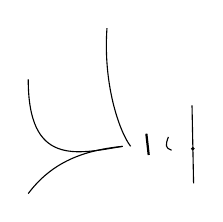
\begin{tikzpicture}[x=1cm,y=1cm]\draw (1,2.1) .. controls (.95,1.4) and (1.15,.8) .. (1.3,.6);\draw (0,1.45) .. controls (0,.35) and (.6,.5) .. (1.2,.6);\draw (0,0) .. controls (.3,.4) and (.7,.55) .. (1.2,.6);\draw[line width=.8pt] (1.5,.76)--(1.53,.49);\draw (1.78,.72) .. controls (1.74,.61) and (1.74,.58) .. (1.82,.55);\draw (2.08,1.12)--(2.1,.13);\fill (2.09,.57) circle (.025);\end{tikzpicture}}}

\uline{il faut et il suffit que} $A$ \uline{possède cette même propriété}.

\uline{Corollaire} (18.8.1\deleted{0}\inserted{3}).-- \uline{Soit} $A$ \uline{un anneau semi-local noethérien. Pour qu'un idéal premier} $\underline p$ \uline{de} ${}^{\mathrm{hs}}A$ \uline{appartienne à} $\operatorname{Ass}({}^{\mathrm{hs}}A)$, \uline{il faut et il suffit que} $\underline p\in A$ \uline{appartienne à} $\operatorname{Ass}(A)$.

Les démonstrations sont les mêmes que celles de (18.6.9), (18.6.10) et (18.6.11) respectivement.

\uline{Proposition} (18.8.1\deleted{1}\inserted{4}).-- \uline{Soit} $A$ \uline{un anneau local ; les propriétés suivantes sont équivalentes} :

a) $A$ \uline{est géométriquement unibranche} (resp. \uline{réduit et géométriquement unibranche}).

b) \uline{Pour toute} $A$-\uline{algèbre locale essentiellement étale} $A'$, $\operatorname{Spec}(A')$ \uline{est irréductible} (resp. \uline{intègre}).

c) $\operatorname{Spec}({}^{\mathrm{hs}}A)$ \uline{est irréductible} (resp. \uline{intègre}).

On se ramène comme dans (18.6.1\deleted{\unsure{1}}\inserted{2}) au cas où $A$ est réduit [\uline{en utilisant (18.8.7.1),}] et l'équivalence de b) et c) se prouve comme dans (18.6.1\deleted{\unsure{1}}\inserted{2}) ; il en est de même du fait que a) entraîne c), en tenant compte de (18.8.7.1) et de la définition d'un anneau local intègre géométriquement unibranche. Enfin pour démontrer que c) entraîne a), gardons les mêmes notations que dans (18.6.1\deleted{\unsure{1}}\inserted{2}) ; il s'agit encore de voir que ${}^{\mathrm{hs}}B$ est intègre. Mais, par (18.8.7), ${}^{\mathrm{hs}}B$ est un anneau local de l'anneau semi-local $B\otimes_A({}^{\mathrm{hs}}A)$, qui s'identifie encore par platitude à un sous-anneau du corps $L$, donc est intègre ; il en est par suite de même de ${}^{\mathrm{hs}}B$, ce qui achève la démonstration.
\margin{?}

\deleted{\unsure{Proposition}} \inserted{\uline{Corollaire}} (18.8.1\deleted{2}\inserted{5}).-- \uline{Soit} $A$ \uline{un anneau \inserted{local} hensélien} (resp. \uline{strictement local})

